\documentclass[conference]{IEEEtran}
\IEEEoverridecommandlockouts

\usepackage{algorithmic}
\usepackage{amsmath, amssymb, amsfonts}
\usepackage{cite}
\usepackage{float}
\usepackage{graphicx}
\usepackage{hyperref}
\usepackage{textcomp}
\usepackage{xcolor}

\def\BibTeX{{\rm B\kern-.05em{\sc i\kern-.025em b}\kern-.08em
    T\kern-.1667em\lower.7ex\hbox{E}\kern-.125emX}}

\begin{document}

\title{Comparative Study of Medical Information Retrieval Approaches}

\graphicspath{ {./images/} }

\makeatletter
\newcommand{\linebreakand}{%
  \end{@IEEEauthorhalign}
  \hfill\mbox{}\par
  \mbox{}\hfill\begin{@IEEEauthorhalign}
}
\makeatother

\author{
    \IEEEauthorblockN{Davin Jason Evan Raharjo}
    \IEEEauthorblockA{\textit{Department of Computer Science} \\
    \textit{and Electronics} \\
    \textit{Universitas Gadjah Mada} \\
    Yogyakarta, Indonesia \\
    davinjasonevanraharjo@mail.ugm.ac.id}
    \and
    \IEEEauthorblockN{Asyraf Nur Ardliansyah}
    \IEEEauthorblockA{\textit{Department of Computer Science} \\
    \textit{and Electronics} \\
    \textit{Universitas Gadjah Mada} \\
    Yogyakarta, Indonesia \\
    asyrafnurardliansyah@mail.ugm.ac.id}
    \and
    \IEEEauthorblockN{Isneyri Arsyadani}
    \IEEEauthorblockA{\textit{Department of Computer Science} \\
    \textit{and Electronics} \\
    \textit{Universitas Gadjah Mada} \\
    Yogyakarta, Indonesia \\
    isneyriarsyadani@mail.ugm.ac.id}
}

\maketitle

\begin{abstract}
    This articles conducts a systematic review of the proposed methodologies according to the PRISMA framework in Medical Information Retrieval (IR), which counts up to the innovations applicable to handling the difficulties of complicated medical jargon, diverse data sources, and privacy requirements. The review examined research on the utilization of adapted IR techniques in medical data analysis, selecting four scholarly articles based on specific criteria. The findings highlight that modified IR models consistently outperformed standard methods in accuracy and efficiency, effectively managing intricate data relationships and addressing vocabulary discrepancies and semantic complexities. These advancements demonstrate that adaptations to IR approaches not only enhance model performance but also improve the precision and relevance of retrieved medical information. By doing so, they contribute significantly to more effective clinical decision-making, providing healthcare professionals and stakeholders with reliable and context-specific insights.
\end{abstract}

\begin{IEEEkeywords}
    medical, information retrieval, medical information systems, PRISMA
\end{IEEEkeywords}

\section{Introduction}

The latest developments in Medical Information Retrieval research have been oriented towards the improvement of direct matching and complemented by the use of innovative methods. The critical role that medical IR plays in healthcare is clear, as it empowers all the stakeholders, ranging from clinicians, researchers, and policymakers, to the possibility to obtain trustworthy, context-relevant, and timely information \cite{McGowan2009}. The scale of this scope embraces the retrieval of different medical-related data sources such as clinical guidelines, diagnostic aids, systematic reviews, and patient-specific data from an array of diverse and yet comprehensive repositories \cite{Cadag2010}. Fast and accurate retrieval (IR) systems need to tackle a lot of issues, and one of them is learning to interpret complicated medical terms, to understand and process the queries, as well as to come up with outputs in the necessary format that would satisfy patients and healthcare specialists.

A notable hurdle in medical IR is grappling with the inherent complexity of the domain \cite{Goeuriot2014}. The specialized medical terminology often features abundant synonyms, abbreviations, and domain-specific jargon that can hinder the retrieval process. Moreover, the confidentiality and sensitivity of patient data necessitate robust mechanisms to ensure adherence to legal and ethical standards \cite{McCarthy2008}. Another obstacle involves managing the diversity of medical data sources, spanning structured databases, semi-structured electronic health records, and unstructured scientific literature \cite{Quamar2020}. Coping with this diversity requires sophisticated approaches to consolidate and analyze data effectively while upholding high precision and recall rates in retrieval tasks.

The objective of this paper is to address these challenges by applying the PRISMA (Preferred Reporting Items for Systematic Reviews and Meta-Analyses) methodology to systematically review and evaluate proposed approaches for improving medical IR. This methodology guarantees a thorough and organized examination of existing literature, emphasizing proposed techniques aimed at mitigating the aforementioned challenges. This study aims to explore improvement in areas such as query expansion, knowledge modeling, and weighting schemes to boost the accuracy and relevance of retrieved medical information.

This research was guided by three key questions: 
\begin{enumerate}
    \item Does it compare different IR techniques within the context of medical information retrieval?
    \item Are the results benchmarked against a standard dataset or compared to other known IR approaches in medicine?
    \item Is there any improvement gained from modifying and/or combining IR methods on enhancing performance?
\end{enumerate}

By addressing these questions, conduct a comprehensive literature review of proposed methodologies in medical IR, providing a critical evaluation of their effectiveness and relevance. The comparative analysis of techniques in various studies highlights the diverse approaches in this domain, while scrutinizing benchmarking methods helps ensure alignment with reliable evaluation metrics. Moreover, delving into innovations that modify or integrate methodologies sheds light on the prospects of hybrid approaches to address current obstacles.

\section{Research Method}

This research uses a literature review approach based on previous research on Medical Information Retrieval (IR). The literature review method used in this study is Preferred Reporting Items for Systematic Reviews and Meta-Analyses (PRISMA) method. This method consists of several steps: identification, screening, eligibility, and inclusion. Figure \ref{fig:PRISMA} shows the steps of the PRISMA method.

\begin{figure}[ht!]
    \centering
    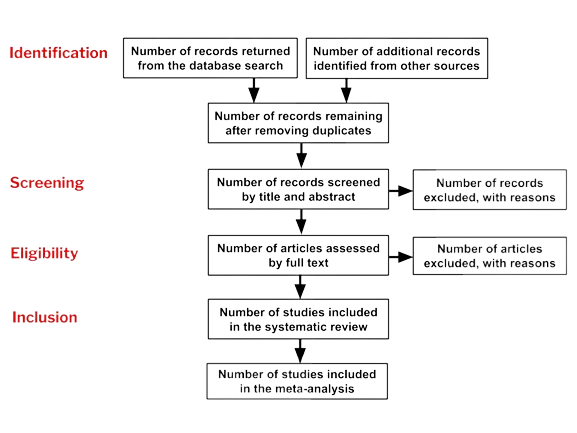
\includegraphics[scale=.4]{PRISMA.png}
    \caption{Steps of the PRISMA method}
    \label{fig:PRISMA}
\end{figure}

The PRISMA (Preferred Reporting Items for Systematic Reviews and Meta-Analyses) method is a standardized framework designed to enhance the transparency and reproducibility of systematic reviews. It is widely utilized to report the selection process of studies systematically and objectively, ensuring that researchers include relevant evidence while excluding unsuitable studies. The method comprises four primary stages: Identification, Screening, Eligibility, and Inclusion, which guide the researcher in narrowing the scope of the studies to be reviewed.

In the Identification stage, all potential studies are collected by searching databases and other sources. At this step, duplicate entries are removed to avoid redundancy. Papers are collected from several journal databases, such as ScienceDirect, Scopus, arXiv, Springer. In order to retrieve the appropriate research papers, we use advanced search feature and keywords based on our main topic. Our query consists of "Information Retrieval", "Medic", "Enhance", where three of them are connected using the AND operator. "Medic" is expanded using the OR operator that links it to "Health" and "Knowledge", which is We also expand "Enhance" term with the same method, adding "Improve" and "Boost" terms. To narrow the studies we found from the query, we set a number of constraints, including English language, their release that is after 2010, research article type, tagged as Computer Science and Engineering domains. The remaining records then proceed to the Screening stage, where their titles and abstracts are evaluated based on predefined inclusion criteria. Studies not meeting these criteria are excluded, with reasons documented for transparency.

In the next stage, Eligibility, full texts of the remaining studies are thoroughly assessed to confirm their relevance and quality. Articles failing to meet the review criteria are excluded, ensuring only high-quality and relevant studies are retained. Finally, in the Inclusion stage, the selected studies form the basis of the systematic review. If applicable, the meta-analysis is conducted using a subset of these studies, providing quantitative insights by synthesizing data from multiple studies. This structured approach ensures rigor and clarity in systematic reviews.

\section{Result}

Using the keywords and constraints for advanced search, we searched and found many studies from the ScienceDirect database, that is 811 results. arXiv, Scopus, and Springer gave much less, respectively 123, 95, and 79. To overcome this, we only picked the top 40 papers from each site, leaving us with 160 studies to proceed. Moving to the next step, we filtered them using a tool named Zotero, which will reduce the number of documents by deleting any duplicates, then excluding any study that doesn't match our topic by its title and abstract. There were 59 studies left after duplicate deletion and further reduced to 19 from the filtering stage.

We manually checked the remaining papers, which found that only 7 of them are appropriate for our topic. Final screening left only 4 studies, where we did an eligibility check on that collection. We got 4 selected researches for the systematic review, including the study conducted by Oh \& Jung (2015), Wang et al. (2016), Zhao et al. (2018), and Balaneshinkordan \& Kotov (2019)

\begin{table}[htbp!]
    \centering
    \caption{Final Documents in Collection}
    \begin{tabular}{|>{\centering}m{2.5cm}|>{\centering}m{2.5cm}|>{\centering\arraybackslash}m{2.5cm}|}
        \hline
        \textbf{Modification} & \textbf{Method} & \textbf{References} \\
        \hline
        Relevance and Expansion Models & Cluster-based External Expansion Model & (Oh \& Jung, 2015) \\
        \hline
        Part-Of-Speech for Term Weighting Scheme & POS-Bag-of-Words, POS-MRF & (Wang et al., 2016) \\
        \hline
        Automation on Knowledge Model Creation & Data-Driven Sublanguage Pattern Mining Method & (Zhao et al., 2018) \\
        \hline
        Probabilistic Framework for Query Expansion & Bayesian Precision Medicine (BPM) & (Balaneshinkordan \& Kotov, 2019) \\
        \hline
    \end{tabular}
    \label{table:PRISMA-Result}
\end{table}

Based on literature data analysis, numerous approaches have been suggested to boost the efficiency of medical Information Retrieval (IR) models. These approaches target enhancement in  various aspects of medical IR, such as query expansion, knowledge modeling, and weighting schemes.

\subsection{Cluster-based Query Expansion using External Collections}

One of the main problems in the field of information retrieval in the medical sector is the shortage of matched vocabulary (synonymy and polysemy phenomena) between a query and documents. One good way to deal with this problem is expanding the query using Pseudo Relevance Feedback (PRF).

The External Expansion Model (EEM) is a PRF method that falls under this category. It constitutes an extension of the Mixture of Relevance Model (MoRM), which mainly deals with the mixing of different document types in the relevant collection in order for the user-issued query to come up with the final retrieval results, the mixture of different query-document relationships. However, it was noticed that these external collections aid EEM only in the case of estimating a co-model.

Oh and Jung \cite{Oh2015} came up with a Cluster-Based External Expansion Model (CBEEM), which is an integration of EEM and Cluster-Based Document Model (CBDM) in order to overcome these limitations. The model sees each external collection as a cluster, which makes it the document model without any extra steps like K-means more accurate.

The trial outcomes illustrated the fact that the CBEEM consistently ranked higher than QL and EEM among all databases. Just to give you an example, for TREC CDS, the CBEEM increased the MAP measure by 15.19\% and NDCG by 10.32\%. In the case of OHSUMED, the CBEEM showed improvements of 15.51\% in MAP and 12.33\% in NDCG. All of these indicate that CBEEM is going to be successfully used for the improvement of the medical information retrieval systems.

\subsection{Part-Of-Speech Term Weighting Scheme}

Current Information Retrieval (IR) systems employ the well-known Bag-of-Words (BoW) approach, but it has a restricted linguistic point of view. Markov Random Field (MRF) is applied, claim word ma'serences are dependent on each other should be helpful to solve this problem. However, it is lim. In the process of the claim, the algorithm that was supposed to assign the weights to the terms within a clique, thus, mainly target those informative terms was potentially overlooking informativeness differences.

To do so, researchers Wang et al. \cite{Wang2016} created a methodology to highlight the biomedical domain for information retrieval by using an automatic Part-Of-Speech term weighting scheme. The POS-BoW and POS-MRF were formed from the term weighing scheme and the already existing BoW and MRF models, respectively.

By introducing the weight calculation algorithm based on supervised learning, they have applied a number of optimization techniques (such as Mean Average Precision (MAP) through the golden section search method and cyclic coordinate descent). Their experimental datasets were composed of Medical Records track (TREC 2011 \& 2012) and Genomics track (TREC 2004). The developed POS-BoW and POS-MRF models were experimentally compared against the already known tf-idf and BM25 methods.

According to the research, the POS-BoW model (with Mean Average Precision (MAP)) showed a rise of 10.88\%, while the POS-MRF model also demonstrated a 13.59\% increase with respect to the traditional BoW and MRF approaches. In the case of the TREC 2004 Genomics track, the POS-MRF model performance improved by around 10.04\% compared to the baseline. The newly proposed POS-driven term weighting scheme outperformed frequency-based and heuristic-based methods, thus proving the potential of the learning algorithm to generate optimal weights effecting the retrieval process of information (IR).

\subsection{Data-Driven Sublanguage Pattern Mining}

Knowledge models serve as structured representations of information within a specific domain, comprising semantic categories as nodes and semantic relationships as edges. These models play a crucial role in converting unstructured textual data into a computationally interpretable format. Existing knowledge models typically depend on machine learning or manually constructed ontologies. As a consequence, it leads to low accuracy in extracting entities and relationships, limited stability and adaptability to new domains due to manual efforts, and ineffectiveness in handling semantic complexity.

To combat this, a new method is introduced by Zhao et al. \cite{Zhao2018} that integrates Natural Language Processing (NLP) and semantic network analysis techniques. This method aims to reveal a sublanguage pattern model within a domain-specific context. It utilizes a novel, bottom-up, context-based approach, combining syntactic analysis and data-driven semantic network analyses to explore semantic relations within a particular corpus.

The evaluation results indicate that the model covers 98\% of entities and 97\% of relationships. Machine annotation achieved a precision of 87\%, recall of 79\%, and an F-score of 82\%. This method shows a promising path to improve the effectiveness of medical information retrieval systems through data-driven sublanguage pattern mining.

\subsection{Bayesian Approach to Incorporate Different Types of Knowledge Bases}

Precision Medicine (PM) \cite{Collins2015} is an ongoing initiative wherein highly personalized healthcare is pursued by providing differential diagnosis of patients at both physiological and molecular levels. The current Information Retrieval (IR) system in Clinical Decision Support (CDS) for Precision Medicine (PM) still cannot optimally utilize data such as genomic and textual data in structured queries. Further, they encounter problems such as a vocabulary mismatch, semantic heterogeneity in medical information, and topic drift during query expansion due to the inclusion of unrelated concepts.

Balaneshinkordan and Kotov developed a new probabilistic framework, Bayesian Precision Medicine (BPM), which uses the Bayesian approach for query expansion \cite{Balaneshinkordan2019}. This approach has a goal to increase the exactness of IR systems in the case of the selection of specific patient articles in CDS systems.

The BPM framework establishes a set of concept extensions for the query via such sources as the Unified Medical Language System (UMLS), Drug-Gene Interaction Database (DGIdb), as well as relevant MEDLINE articles first. This is done by assigning prior probabilities for co-occurring terms and genomic context while tying textual and genomic query details together using Bayesian inference.

On analyzing the TREC 2017 Precision Medicine dataset, it is revealed that BPM, with a total recall of 0.4929 against the current system's 0.4593, has shown a marked improvement in system performance. Important findings brought to the fore include superior concept performance of the sources from MEDLINE and the finer accuracy achieved by the disease and gene characteristics.

\section{Discussion}

The review conducted in this study analyzed the Medical Information Retrieval (IR) by the different methodologies via the PRISMA framework to highlight the difficulties. The selected studies offer in-depth analysis of how the changes in information retrieval methods have had an impact on the retrieval of medical information. The part presents the findings on the three main research questions (RQs) envisaged at the very outset of the research.

\subsection{RQ1: Comparison of Different IR Techniques in Medical Information Retrieval}

The report description was about several new IR techniques for the healthcare industry. It provides solutions to problems like the mismatch of vocabularies, the complexity of the semantics, and the need for integrating the multiple data sources in the domain of medicine. The studies which are analyzed used different techniques, including the Cluster-Based External Expansion Model (CBEEM), Part-Of-Speech (POS) term weighting schemes, data-driven sublanguage pattern mining, and Bayesian Precision Medicine (BPM).

CBEEM got really good results in research by actually acquiring model data from databases and used them to make the model more relevant after absorbing the vocabularies' mismatch. Like that, the POS term weighting scheme IR system gains accuracy because the linguistic context is taken into consideration, which is particularly important in the medical setting where the terminologies can differ. The data-driven sublanguage pattern mining technique efficiently showed a way of learning the nature and language leadership of new entities and relationships. Within the BPM framework, the Bayesian methods were used to integrate genomic and textual data, and hence this made retrieval of the information relevant for clinical decision-making easier.

Of the two, the direct comparison of these techniques suggests the more successful modified IR methods often perform better than traditional tactics, which shows the real need of special applications in the field of medicine.

\subsection{RQ2: Benchmarking Against Standard Datasets and Known IR Approaches}

The systematic review carried out in this research was to overcome the problems encountered in Medical Information Retrieval (IR) by evaluating various methods using the PRISMA framework. The findings of the specific experiments provide the reader mainly with an understanding of the effectiveness of transformed IR techniques in the field of medical information retrieval. This part is concerned with disclosing the findings of the study connected to the three main research questions (RQs) that were earlier asked.

The studies that were examined in this lit review used different benchmarking methods to gauge the performance of their IR systems. One example of this is when CBEEM's relative performance was compared to conventional methods such as Query Likelihood (QL) and the initial External Expansion Model (EEM), in which the results showed that there was a significant increase in MAP and NDCG by means of both TREC CDS and OHSUMED sets, respectively. Similarly, the POS term weighting models were also compared to established baselines such as tf-idf and BM25, which exhibited noticeable improvements in MAP.

BPM Framework also made use of the TREC 2017 Precision Medicine dataset for measuring the performance it was able to achieve, arriving at the conclusion that the new system is very strong compared to existing systems. These benchmarking activities not only prove the efficacy of the hypothesized methods but also guarantee that the advances made are indeed based on a reliable measure of evaluation. The consistent enhancements throughout these various works are poignant evidence for the thesis idea that adapting IR methods is the only way to address the peculiar problem of medical information search.

\subsection{RQ3: Improvement from Modifying and/or Combining IR Methods}

The review indicates that modification and combination of existing IR methods resulted in very good performance. The inclusion of external collections in CBEEM, the linguistics in the POS term weighting scheme, and a novel data-driven approach in sublanguage pattern mining are all examples of how modifying established methods can give better outcomes in the medical field.

Furthermore, the probabilistic method described in the BPM framework for query expansion is the case that throwing together different types of knowledge bases can be done by effectively dealing with vocabulary mismatch and semantic heterogeneity. The feedback from these studies is that mixed methods of hybrid models can deliver the accuracy and relevance of the extracted medical data and can be one of the ways to break already existing borders of IR methodologies.

Summing up, the results of this systematic review are the turning point for IR technology to evolve into a highly specialized medical field. The development featured in this study not only increases the functionality of IR systems but also perks up more efficient decision-making by healthcare providers; therefore, end-users and stakeholders are satisfied.

\section{Conclusion}

The literature review was based on the studies that were conducted to use modified information retrieval (IR) techniques in medical data analysis. The PRISMA method was applied, and four scholarly articles were selected as per the given criteria. The findings of the study point out that the revised IR models were practically always found to bring about marked advantages in terms of performance when compared to the methods that are standard. They also had capabilities in data dependency management, especially in handling vocabulary discrepancies and semantic complications.

As news published suggests, the changes to IR methods can be looked at from both the side of model effectiveness and the improved accuracy of information retrieval; thus, the medical field will also have better clinical decision-making protocols.

\bibliographystyle{ieeetr}
\bibliography{references}

\end{document}
